\section{DDK}

dc_create_proxy()里有一个重要操作就是将原来的驱动变成proxy.so驱动。

只有创建新devhost进程的驱动才有create()方法,创建一个proxy设备。
devhost proxy设备的add_device不会回到dc里。直接在devhost_device_add握手结束。


sys -> kpci -> achi 设备关系示意图

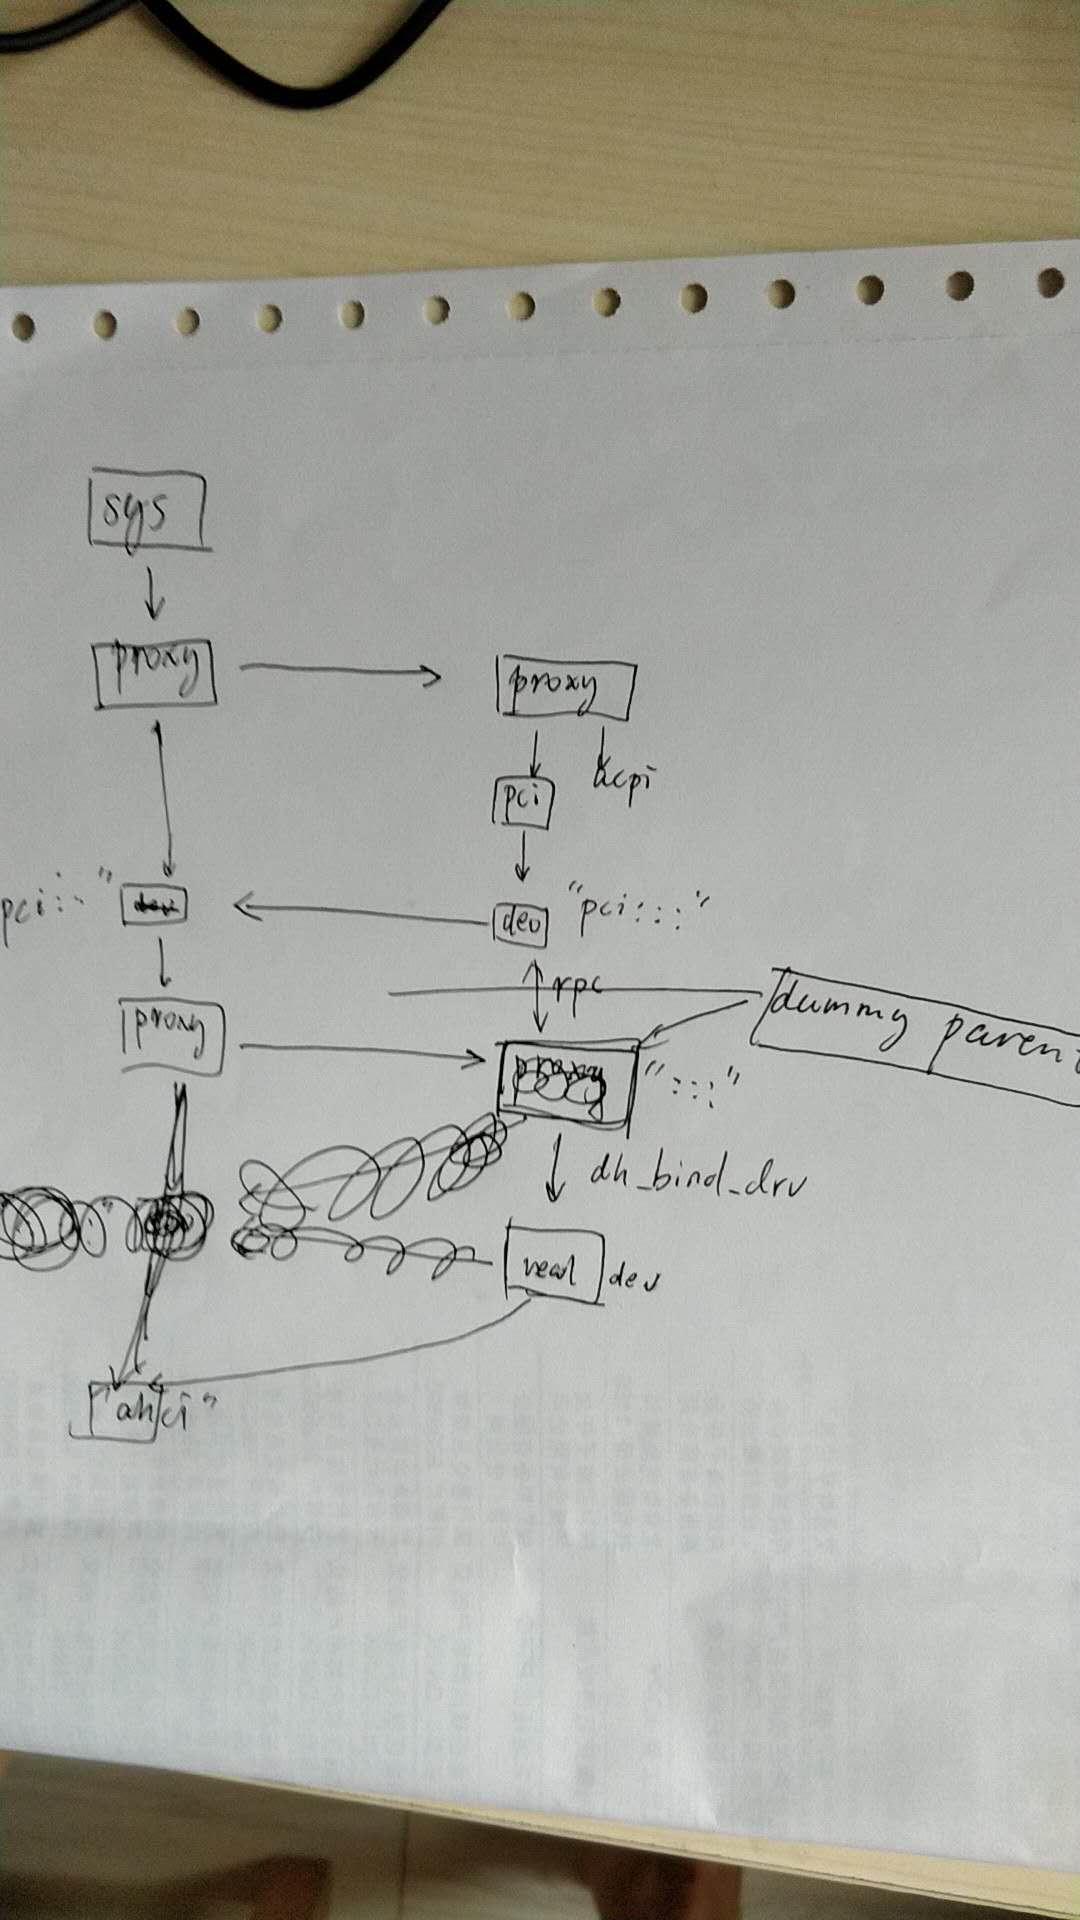
\includegraphics[scale=0.3]{devdrv.jpeg}

\begin{verbatim}
ZIRCON_DRIVER_BEGIN会定义
__zircon_driver_rec__ {
    /* .ops = */ &(Ops),
    /* .driver = */ NULL,
    /* .log_flags = */ 7, /* DDK_LOG_ERROR | DDK_LOG_WARN | DDK_LOG_INFO */
}


__zircon_driver_note__ {
    zircon_driver_note_t note;
    zx_bind_inst_t binding[BindCount];
}
也就是
  .note = {
    /* .namesz = */ sizeof(ZIRCON_NOTE_NAME),              
    /* .descsz = */ (sizeof(object) -                       
                         sizeof(zircon_driver_note_header_t)), 
    /* .type = */ ZIRCON_NOTE_DRIVER,                      
    /* .name = */ ZIRCON_NOTE_NAME,  
    
    /* .flags = */ ZIRCON_DRIVER_NOTE_FLAGS,                    
    /* .bindcount = */ (BindCount),                             
    /* .reserved0 = */ 0,                                       
    /* .name = */ #Driver,                                      
    /* .vendor = */ VendorName,                                 
    /* .version = */ Version,            
  }

BI_MATCH_IF(EQ, BIND_PROTOCOL, ZX_PROTOCOL_INTEL_GPU_CORE)
expands to:

BINDINST(COND_##EQ,OP_MATCH,0,BIND_PROTOCOL,ZX_PROTOCOL_INTEL_GPU_CORE)
#define BINDINST(c,o,a,b,v) \
    { (((c)&0xF)<<28)|(((o)&0xF)<<24)|(((a)&0xFF)<<16)|((b)&0xFFFF),(v) }

dc_is_bindable(drv, dev->protocol_id,dev->props, dev->prop_count, true)
    drv->binding指向的是zx_bind_inst_t


acpi 会导致kpci被bind, 因为acpi protocol id 是ZX_PROTOCOL_PCIROOT.
kpci会match这个protocol id.

一个驱动发布设备时,会指定protocol id, 如果别的驱动匹配这个protocol id, 则会加载该驱动。

i915的match需要BIND_PCI_DID。这个只有kpci.c: pci_init_child()才会设置。
\end{verbatim}


